\chapter{\emph{Model Judge}: A Practical Use Case of ATD}
\label{cha:modeljudge}

Due to the wide usage of process models in organizations, correctness and
quality of models directly influences the correct execution of processes.
However, research has shown that industrial process models often
contain errors\cite{citation needed}.

Automating the detection of \emph{syntactic} errors is a common feature in 
modelling software. However, other error types more closely related to the
natural language sections of the process model are not checked. Part of this
Master thesis' work consisted in exploring a practical application of Annotated
Textual Descriptions by designing the main algorithm behind \emph{Model
  Judge}\cite{citation needed}. \emph{Model Judge} is a web platform supporting
students in the creation of business process models by automatically detecting
and reporting the most common sources of \emph{semantic} and \emph{pragmatic}
errors in modeling The motivation behind the platform and its functionalities
are discussed in
Sections~\ref{sec:modeljudge_description}~and~\ref{sec:modeljudge_tour}.


The algorithm, which is described in detail in
Section~\ref{sec:modeljudge_approach} is based on the automatic computation of
alignments between process model and textual descriptions (covered in
Section~\ref{sec:background_alignments}). However, it has been adapted to use
ATDs (covered in Chapter~\ref{cha:atd}) instead of plain natural language text.

The \emph{Model Judge} platform has been used as the main modeling tool as
part of two Computer Science courses: One in Denmark's Technical University
(DTU) and another in the Catholic University of Santa Mar\'ia (UCSM).
Section~\ref{sec:modeljudge_results} defines the experimental setting and
analyzes the results obtained from the modeling sessions.

\section{The \emph{Model Judge} Platform}
\label{sec:modeljudge_description}
 

% Explain the use case: What does \emph{Model Judge} do?

\emph{Model Judge} is a web platform designed to provide diagnostics regarding
issues on \emph{syntactic}, \emph{pragmatic} and \emph{semantic} quality in
business process diagrams. Students are presented with a statement describing a
business process in natural language, and are asked to model the corresponding
diagram.

The framework behind \emph{Model Judge} is based on computing an alignment
between the process model diagram to be evaluated and a reference textual
description, which is an ATD based on the exercise's statement. This ATD is
generated only once, with intervention from the course instructors, and can be
used to support multiple students simultaneously.


\subsection{Diagnostics}

\emph{Model Judge} is based on computing quality diagnostics on business process
models. Instead of providing the user with a difficult to interpret numerical
score, we believe more detailed feedback helps students and contrinbutes to
continuous self-improvement.

By observing the grading process of several modeling courses, we have
established a set of diagnostics that are suitable for being computed
automatically. We have split these diagnostics in three different categories:
\emph{Syntactic} diagnostics consider the structure of the model.
\emph{Pragmatic} diagnostics verify the phrasing of the process model labels and
can be tuned to enforce certain grammatical rules. Finally, \emph{semantic}
diagnostics check if there is no missing information from the underlying process
and all the information provided is relevant. Next, we detail the concrete
diagnostics for the three aforementioned types.

\subsubsection{Syntactic Diagnostics}

A good process model should have a clear and unambiguous control flow.
Syntactic diagnostics identify common patterns that typically result in
less understandable and maintainable process models.

\begin{description}
\item[Gateway Reuse and Implicit Gateways.]{Gateway reuse re\-fers to a gateway
    that acts both as a \emph{split} (more than two ouptuts) and a \emph{join}
    (more than two inputs). Implicit Gateways exist when an activity has
    multiple input or output flows. The semantics for these two constructs are not
    clear and can lead to hidden modeling errors. Because of that, avoiding gateway reuse and implicit
    gateways is a well-known best practice in business process models~\cite{MendlingRA10,BernsteinS15,Haisjackl2018}.}
\item[Non-Natural Loops.]{Due to their similarity, some desirable properties of
    program's control flow graphs are also relevant in the context of process
    model diagrams. Ideally, process models should contain only of \emph{Natural
      Loops}. That is, there is only a single way to enter the loop. 
      %That is, all loops should jump back to the beginning of a \emph{SESE} (Single-Entry, Single-Exit) region of the process~\cite{MendlingRA10}.
      We have observed non-natural loops are a common pattern among novice students.}
\item[Soundness.]{A well-known desirable property of process models is {\em soundness}~\cite{AalstHHSVVW11}, which guarantee the process model is free from livelocks, deadlocks, and other anomalies that can be detected without domain knowledge.}
\end{description}

\subsubsection{Pragmatic Diagnostics}

Process model diagrams define a large portion of their semantics using natural
language. It is desirable to restrict the language to a strict writing style (e.g, the {\em verb-object} rule in~\cite{MendlingRA10}, G6), in
order to avoid ambiguous phrasing~\cite{Leopold0M12}. A simple and strict style is also important
when considering automatic analysis of the process model language. For example, 
while it is acceptable in the text to include the sentence: \emph{``The latter is then
responsible for taking a sample to be analysed in the lab later''}, having that 
sentence as an activity label in the process model adds unnecessary complexity,
since the aim is to have label text to be as simple as possible.

Previous studies \cite{mendling2010activity, Leopold0M12, leopold2013detection,PittkeLM16} have
established the common structures in label descriptions. However, these
structures are not always followed by novice students. Because of that, an
automatic detection of invalid writing styles is beneficial for student
self-improvement.

\subsubsection{Semantic Diagnostics}

A process model diagram has to communicate the semantics of the underlying
process in a clear and unambiguous way. 
All the information provided has to be
correct, and in the right order. On the other hand, unnecessary information
introduces noise that can generate confusion. Semantic diagnostics help enforcing these properties on the process model.

\begin{description}
\item[Missing/Unnecessary activities.]{This problem arises when a relevant activity of the
    process is omitted from the process model, or symmetrically when additional activities are added which are either wrong or add no relevant
    information. This can be caused by an
    oversight or a poor understanding of the process being modeled.}
  
% \item[Unnecessary activities.]{This problem occurs when additional activities
%     are added to the process, which are either wrong or add no relevant
%     information.}

\item[Missing/Unnecessary Roles.]{When process models use role information,
    such as swimlanes in BPMN, the same diagnostics of \emph{missing} 
    and \emph{unnecessary} roles can be applied as well, to ensure
    all the relevant actors are properly modeled.}
  
\item[Control-Flow Consistency.]{All the information in the process model
    should be consistent with the control flow of the process being described. 
    If some temporal relationship described in the text is not accurately incorporated in the process model, then a control-flow consistency violation would be communicated to the novice modeler.}  
%     the activities
%     describing that part of the text should be in the correct position in 
%     the control flow graph.}
\end{description}

\section{A Tour through \emph{Model Judge}}
\label{sec:modeljudge_tour}

The \emph{Model Judge} can be accessed using any modern web browser at
\url{http://modeljudge.cs.upc.edu}. It is designed both for helping students in
the process of creating a process model, and instructors in the task of
designing modeling activities in an agile way. \todo{Should I make it explicit that I didn't do the application?}

The application requires registration, and users with the \emph{instructor} role
are able to create and manage courses. However, the functionality to include new
exercises is restricted to the developers of the application.

All registered users are able to access the exercise list and attempt solving
any of them. After selecting an exercise, the user is brought to the modeling
view, which is displayed in Figure~\ref{fig:validation}. In the modeling view,
the user has access to a textual description of the process, and a BPMN editor.

During the exercise, students can use the \textbf{Validation} functionality to
obtain aggregated diagnostics about the process model, for example, how many
unnecessary activities it contains. A more detailed version is the \textbf{Complete
  Validation}, which offers more fine-grained information about the diagnostics,
such as the exact labels of the unnecessary activities in the process model.

Finally, for users that allow it during registration, analytics are enabled. The
analytics functionality which is built into the platform periodically records
snapshots of the student's process model for the duration of the validation
session. Additional snapshots are created each time a user performs a
\textit{validation} or \textit{complete validation}.
Section~\ref{sec:modeljudge_results} describes the analysis perform on the
analytics data.

\begin{figure}[htb]
  \centering
  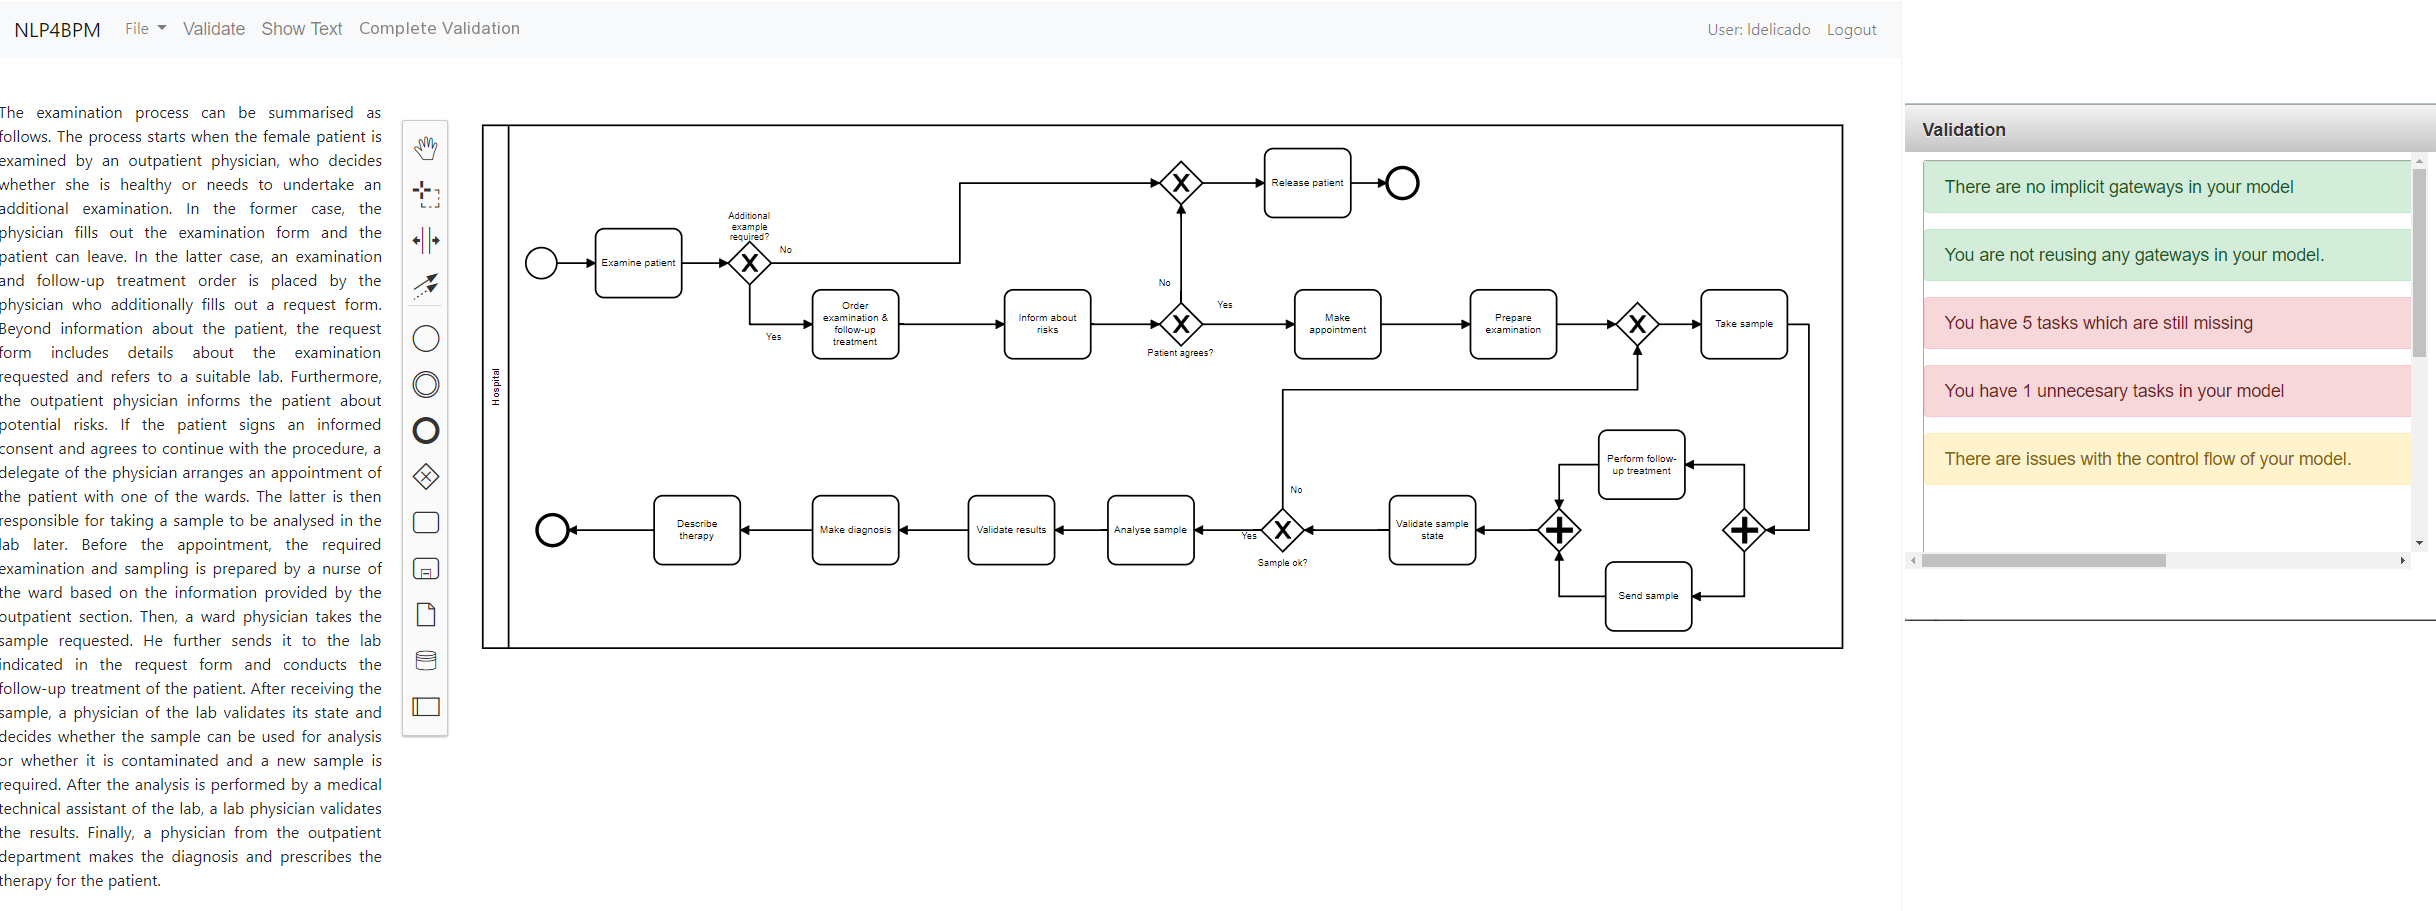
\includegraphics[width=\textwidth]{figures/validation}
  \caption{Model Judge modeling view}
  \label{fig:modeljudge_validation}
\end{figure}



\section{Approach}
\label{sec:modeljudge_approach}

At the Model Judge's core, there is the algorithm that produces a list of
diagnostics for their current business process model. The design and
implementation of this algorithm was done as part of this Master Thesis.

In Figure~\ref{fig:modeljudge_overview}, we can see a BPMN model of the
diagnostic generation process. The inputs to the system are the \emph{Textual
  Description}, which corresponds to the exercise statement, and the
\emph{Process Model} created by the student.\todo{Change start event label to
  ``Student clicks validation button''?}. First, the textual description is
analyzed by the Text Annotation module to automatically produce an Annotated
Textual Description. The ATD is then completed with human intervention to
include the domain expertise not available to the NLP algorithms. Additionally,
 the \textit{Alignment} between the process model elements, such as activities
 or gateways and the annotations in the ATD is established. Finally, using all
 the previous information, the process model is checked against a textual
 description by the \emph{Diagnostics} module.  

 \todo{Finish describing the approach once it's clearer what we will explain in
   Chapter 3}

%- How are ATDs used in \emph{Model Judge}

%- How are the alignments used in \emph{Model Judge}

\begin{figure}[htb]
  \centering
  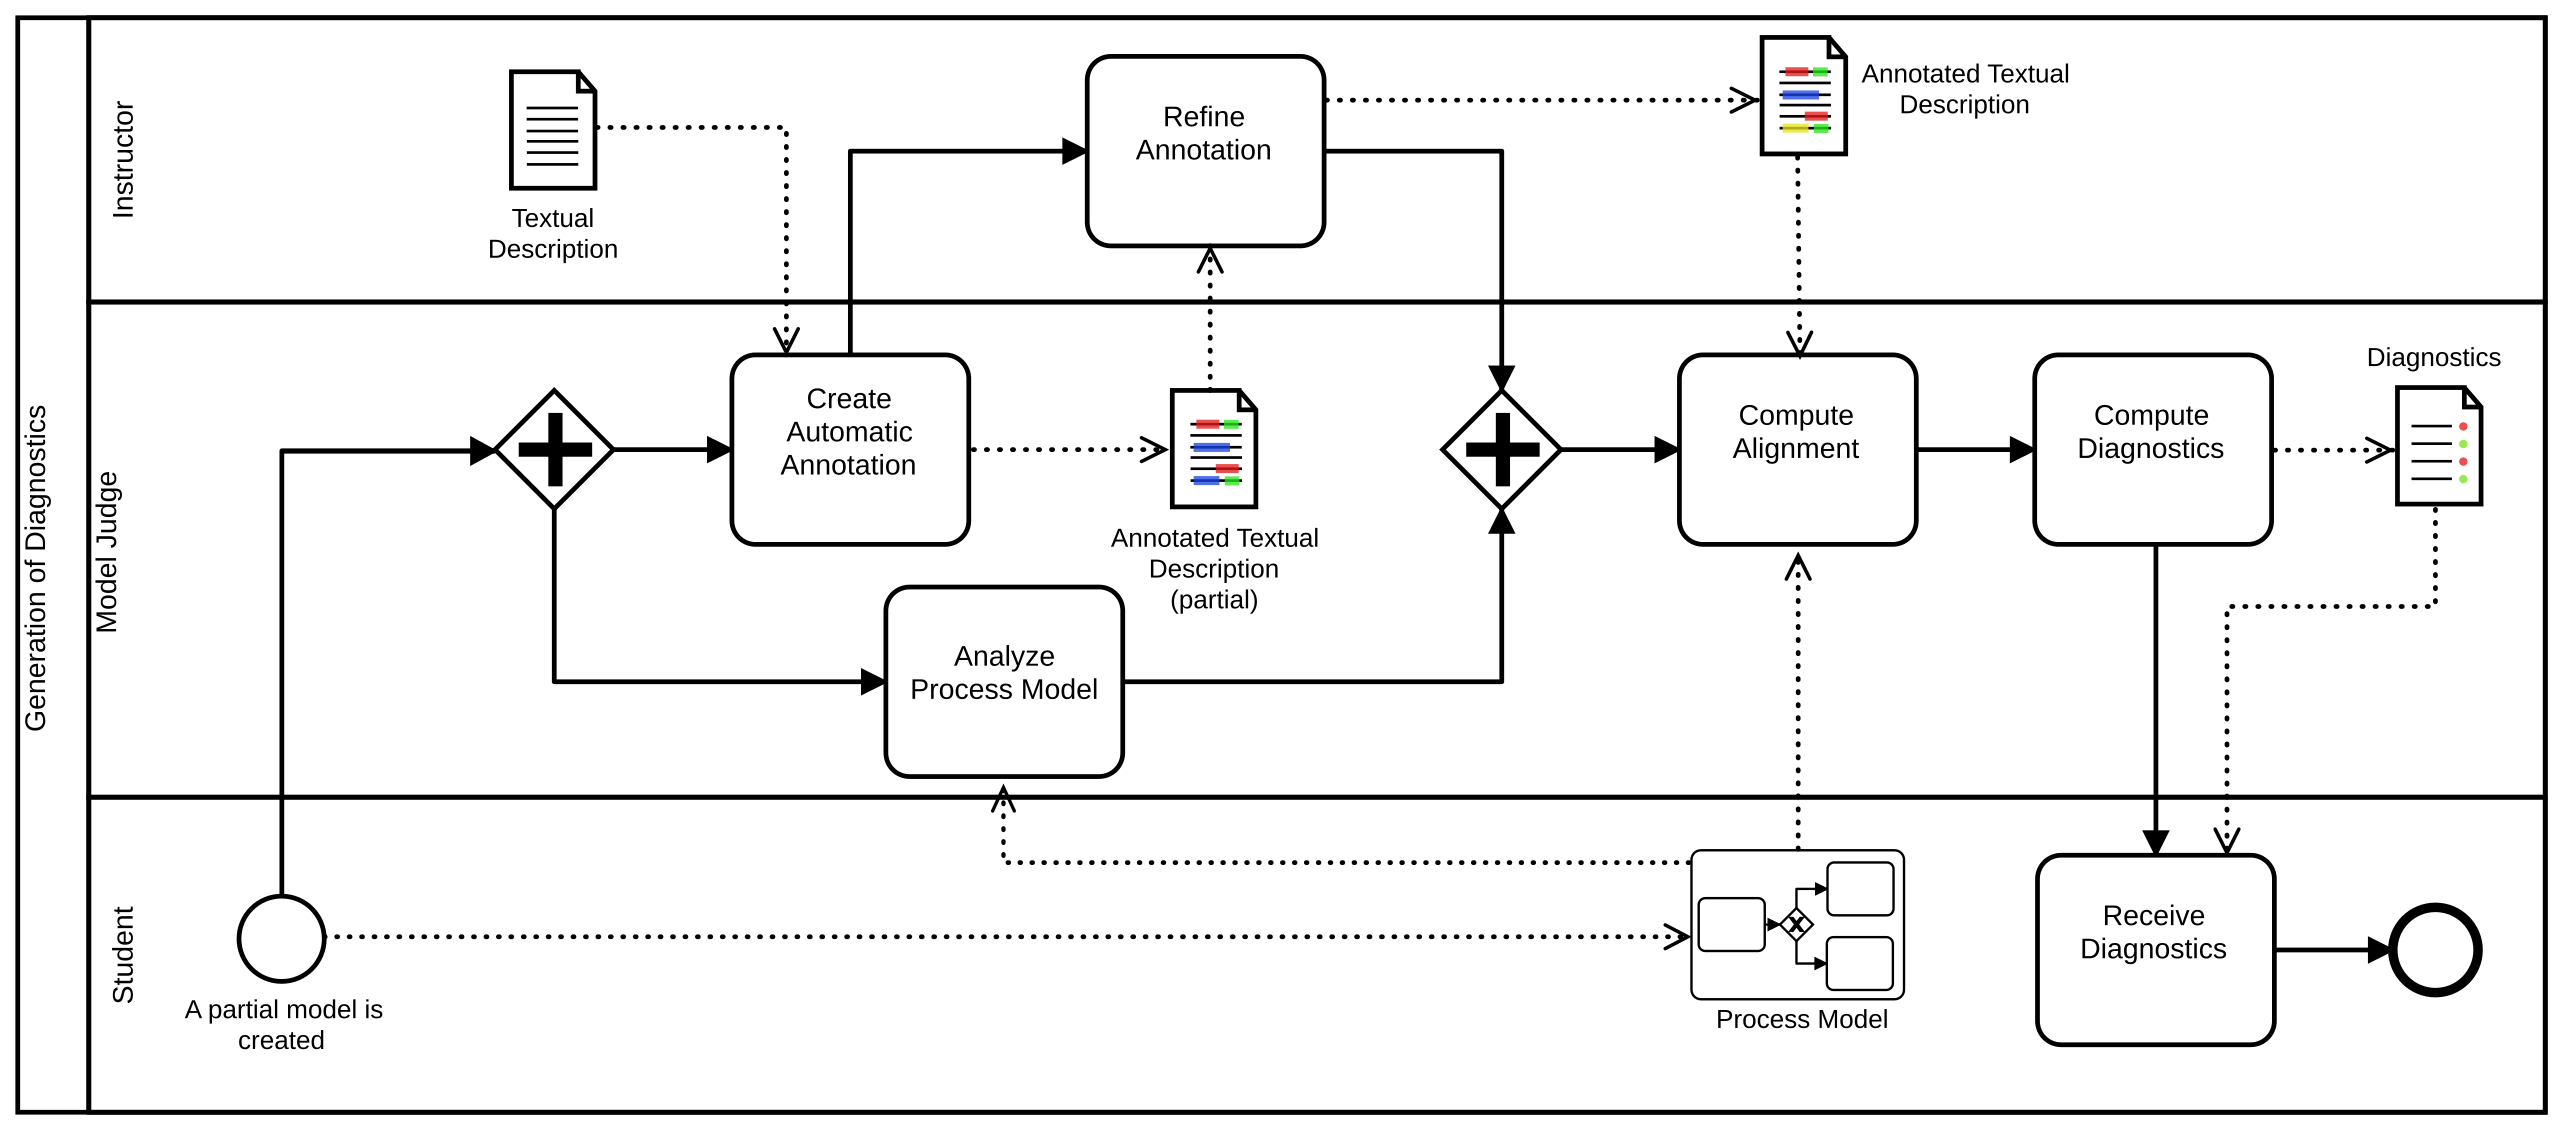
\includegraphics[width=\textwidth]{figures/overview_bpmn}
  \caption{\emph{Model Judge} process overview}
  \label{fig:modeljudge_overview}
\end{figure}

\section{Experiments}
\label{sec:modeljudge_results}

\todo{Describe dataset in further detail}

The \textit{Model Judge} has been tested in two separate modeling courses. The first was performed on the Technical University of Denmark (DTU) during February 2018. as part of a graduate course on business process management. 
The second course was performed at the Catholic University of Santa Mar\'ia (UCSM) in Peru during March 2018 as part of a practical session in the Business Process Management course in the Computer Science degree.

In order to validate how the \textit{Model Judge} helps novice modelers, we performed two evaluations.  The first one consisted in analyzing the recorded data from the modeling sessions (Sect. \ref{sec:data_analysis}). The second evaluation arises from a survey that was handed to the students at the end of the modeling course (Sect. \ref{sec:questionaires}). Below, we detail the results obtained in both evaluations.

\subsection{Analysis of the Modeling Session Data}
\label{sec:data_analysis}
There were substantial differences in the setting of the two courses. On the DTU course, students were allowed to complete the exercise at home without a time limit. On the other hand, the UCSM course consisted in two exercises that had to be completed in a two-hour session.
%Additionally, in first UCSM exercise, the students were discouraged to use the complete validation functionality until the end of the exercise.
Additionally, some technical issues affecting DTU students were corrected before the UCSM course. Despite the differences, we believe the information recorded is still relevant for the analysis we present in this session. 
%However, we believe a better controlled experiment would be necessary in order to draw more statistically robust conclusions.
%\todo{[JS: Please check the above paragraph.]}

% For the students that allowed the recording of their data for research purposes 
For every student, we stored periodically (every minute) information for the whole modeling session. Additionally, information was also saved each time the user performed a simple or complete validation. In particular, we recorded a total of 8410 intermediate models for 72 students. For the snapshots, we stored: \textit{(i)} A unique user identifier. \textit{(ii)} The process model in BPMN (XML) format. \textit{(iii)} The timestamp of the snapshot. \textit{(iv)} The type of information: automatic, validation or complete validation. \textit{(v)} The validation results of our tool for the particular process model. Note that the validation results were computed for all snapshots, despite the students only seeing the ones they explicitly requested. 
After the modeling course ends, we analyzed the snapshots with the aim of observing the evolution of the number of validation errors during the modeling sessions. The dataset used to perform this analysis can be found in the following address: \texttt{\url{http://www.cs.upc.edu/~pads-upc/ModelJudgeData.zip}}.

\subsubsection{Modeling Behaviours}

By manual inspection, we identified several modeling profiles when analyzing the sessions data.
Figure~\ref{fig:profiles} shows a representative for each of the identified profiles, when plotting number of validation errors vs.
time (in seconds)\footnote{There exists few outlier profiles that do not match any of the three representatives shown in Fig.~\ref{fig:profiles}.}.
An instructor can have a good summary of the student evolution by looking at these student's plots:
\emph{(i)} The first group is composed of students that frequently use the validation and complete validation functions, and ended up with almost no bad diagnostics. This group corresponds to $19.0\%$ of the students ($30.4\%$ in the DTU course and $12.5\%$ in the UCSM course).
\emph{(ii)} The students from the second group frequently use the simple validation, however, only check the complete validation at the end of the session. The final amount of bad diagnostics for this group is comparable to the previous one. This group corresponds to $60.3\%$ of the students ($56.5\%$ in the DTU course and $62.5\%$ in the UCSM course).
\emph{(iii)} The students from the third group started working on the exercise but finished before fixing the majority of bad diagnostics. We have observed that the students in this group performed substantially less validations. This group corresponds to $20.6\%$ of the students ($13.0\%$ in the DTU course and $15.8\%$ in the UCSM course).

\begin{figure}
  \centering
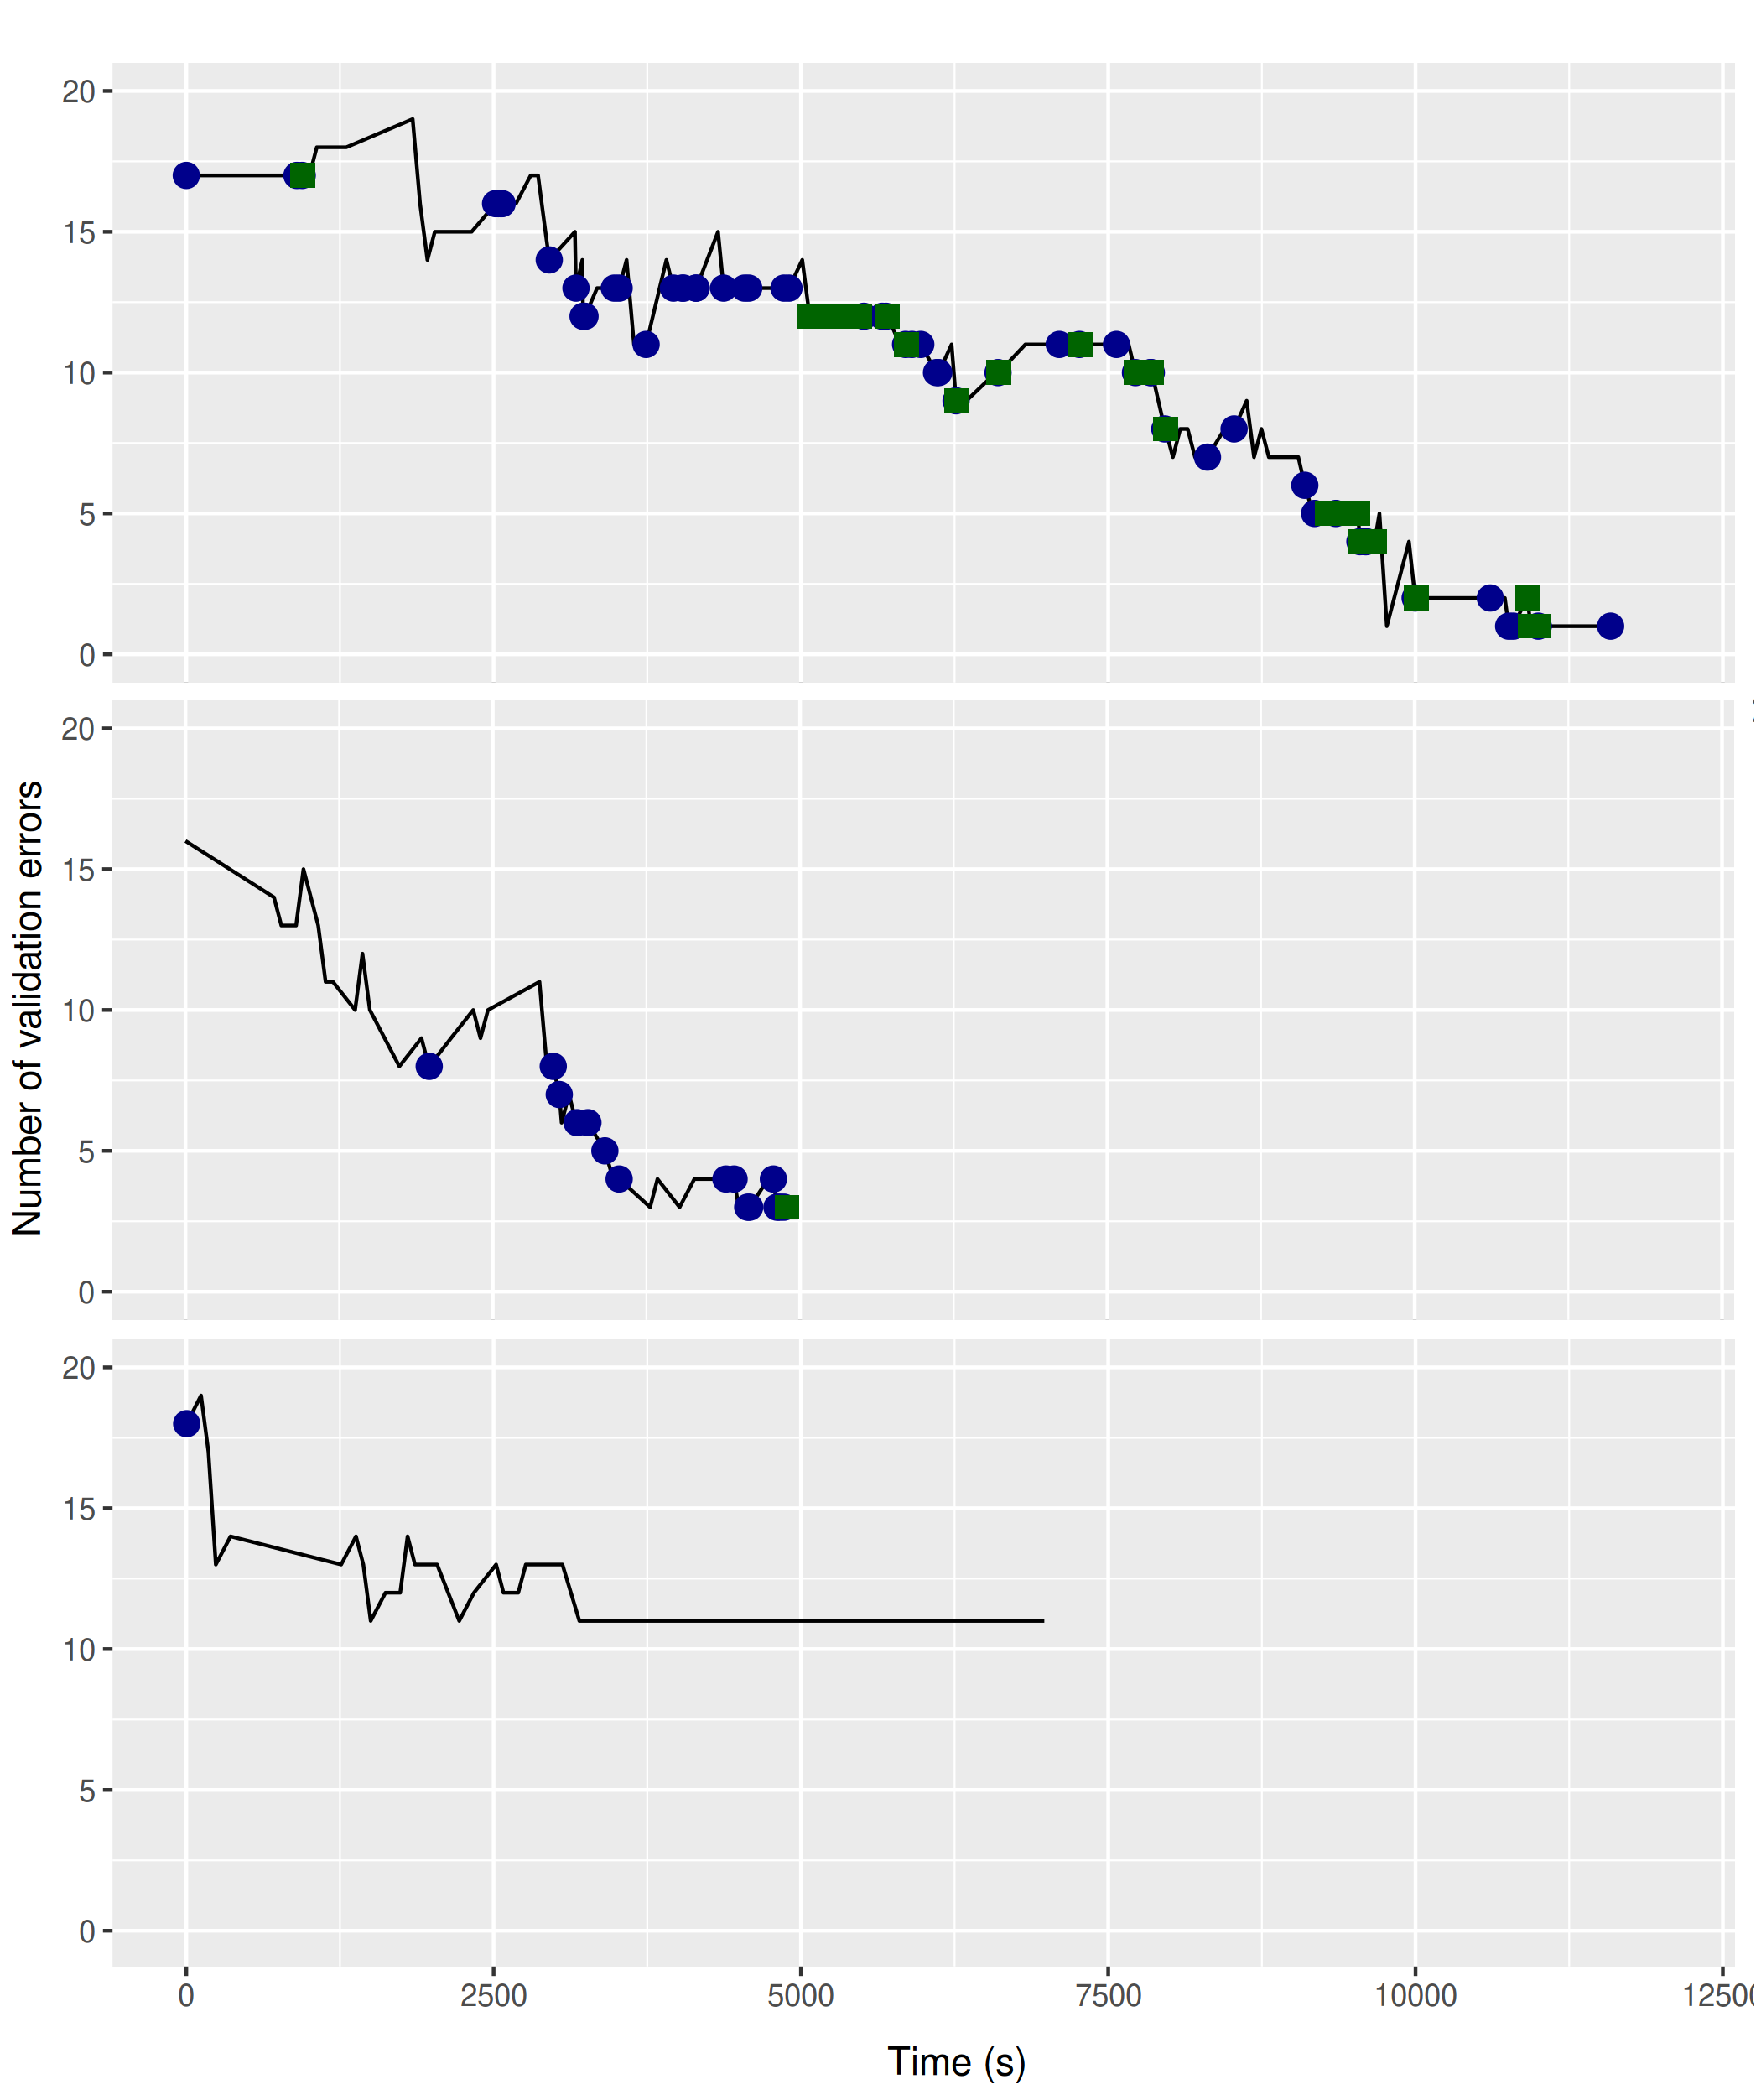
\includegraphics[width=0.85\textwidth]{figures/results/profiles.png}
\caption{Three characteristic behaviors observed in the modeling sessions. The blue circles represent simple validations, while green squares denote complete validations.}
\label{fig:profiles}
\end{figure}

\subsubsection{Evolution of Diagnostic Types}


\begin{figure}
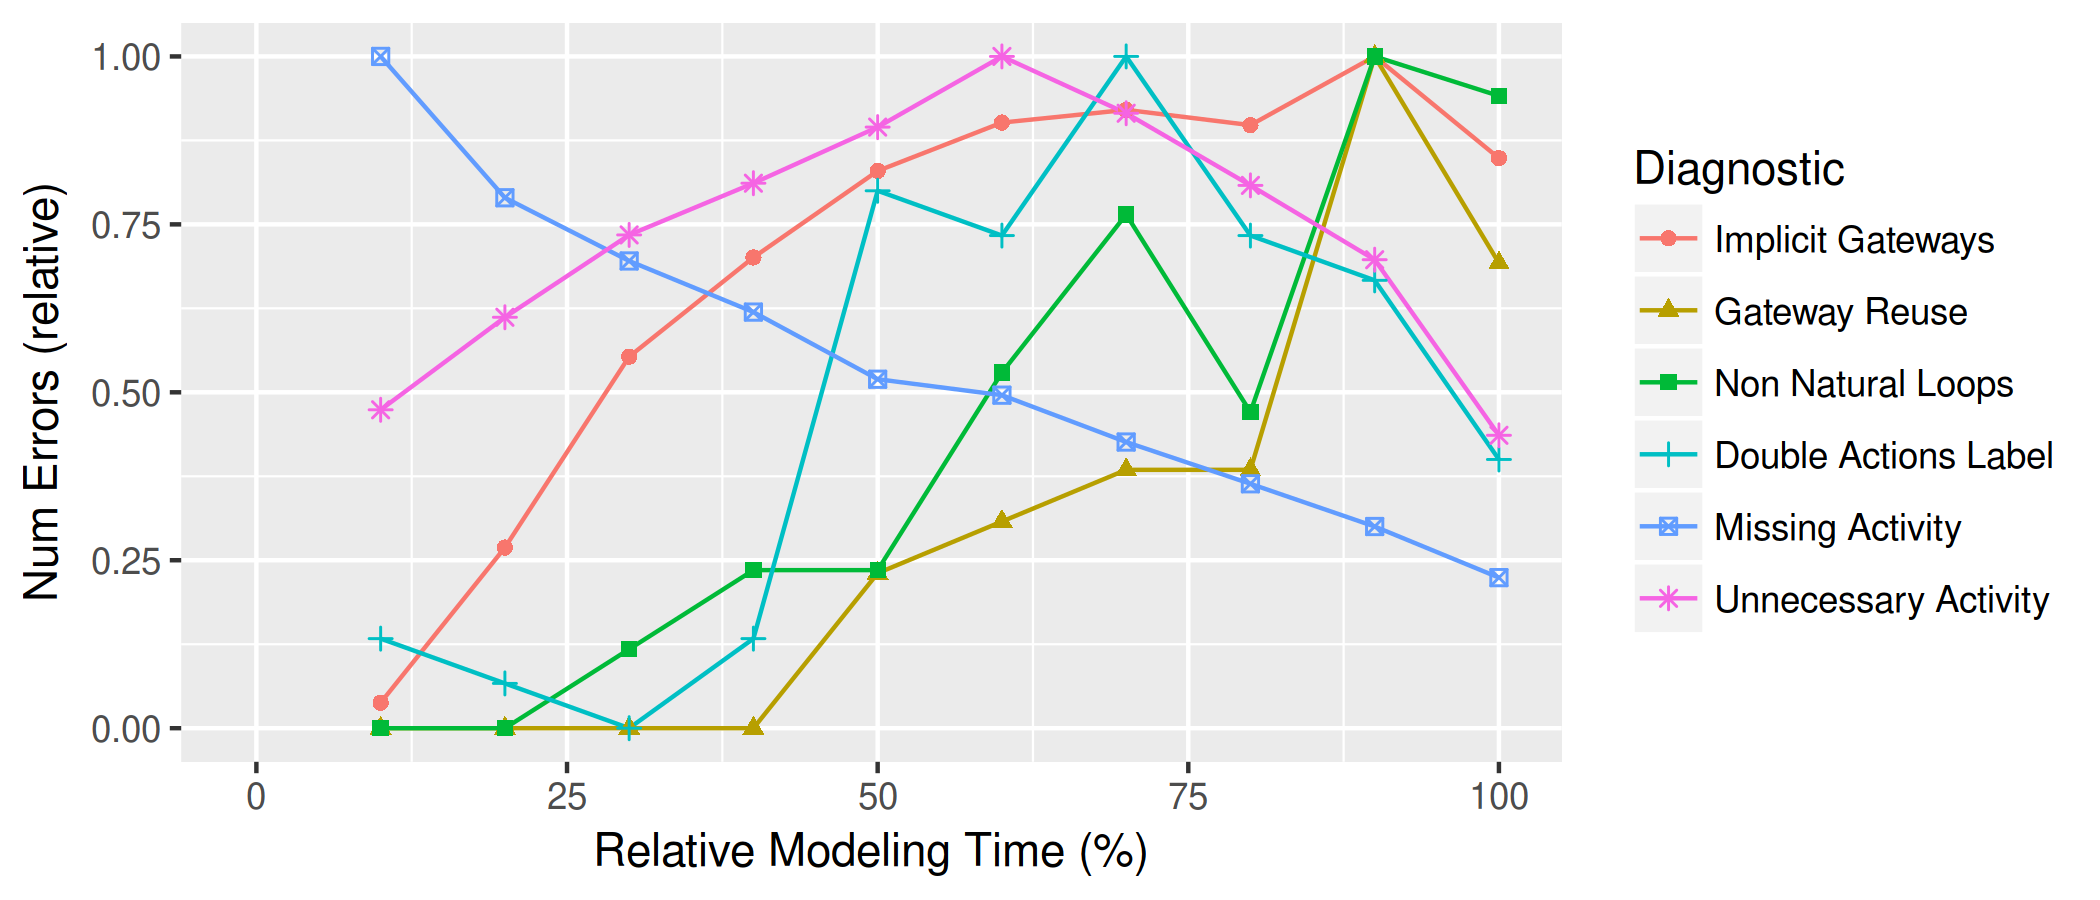
\includegraphics[width=\textwidth]{figures/results/evolution}
\caption{Evolution of the diagnostic types for the modeling session.}
\label{fig:error_evolution}
\end{figure}
\begin{figure}

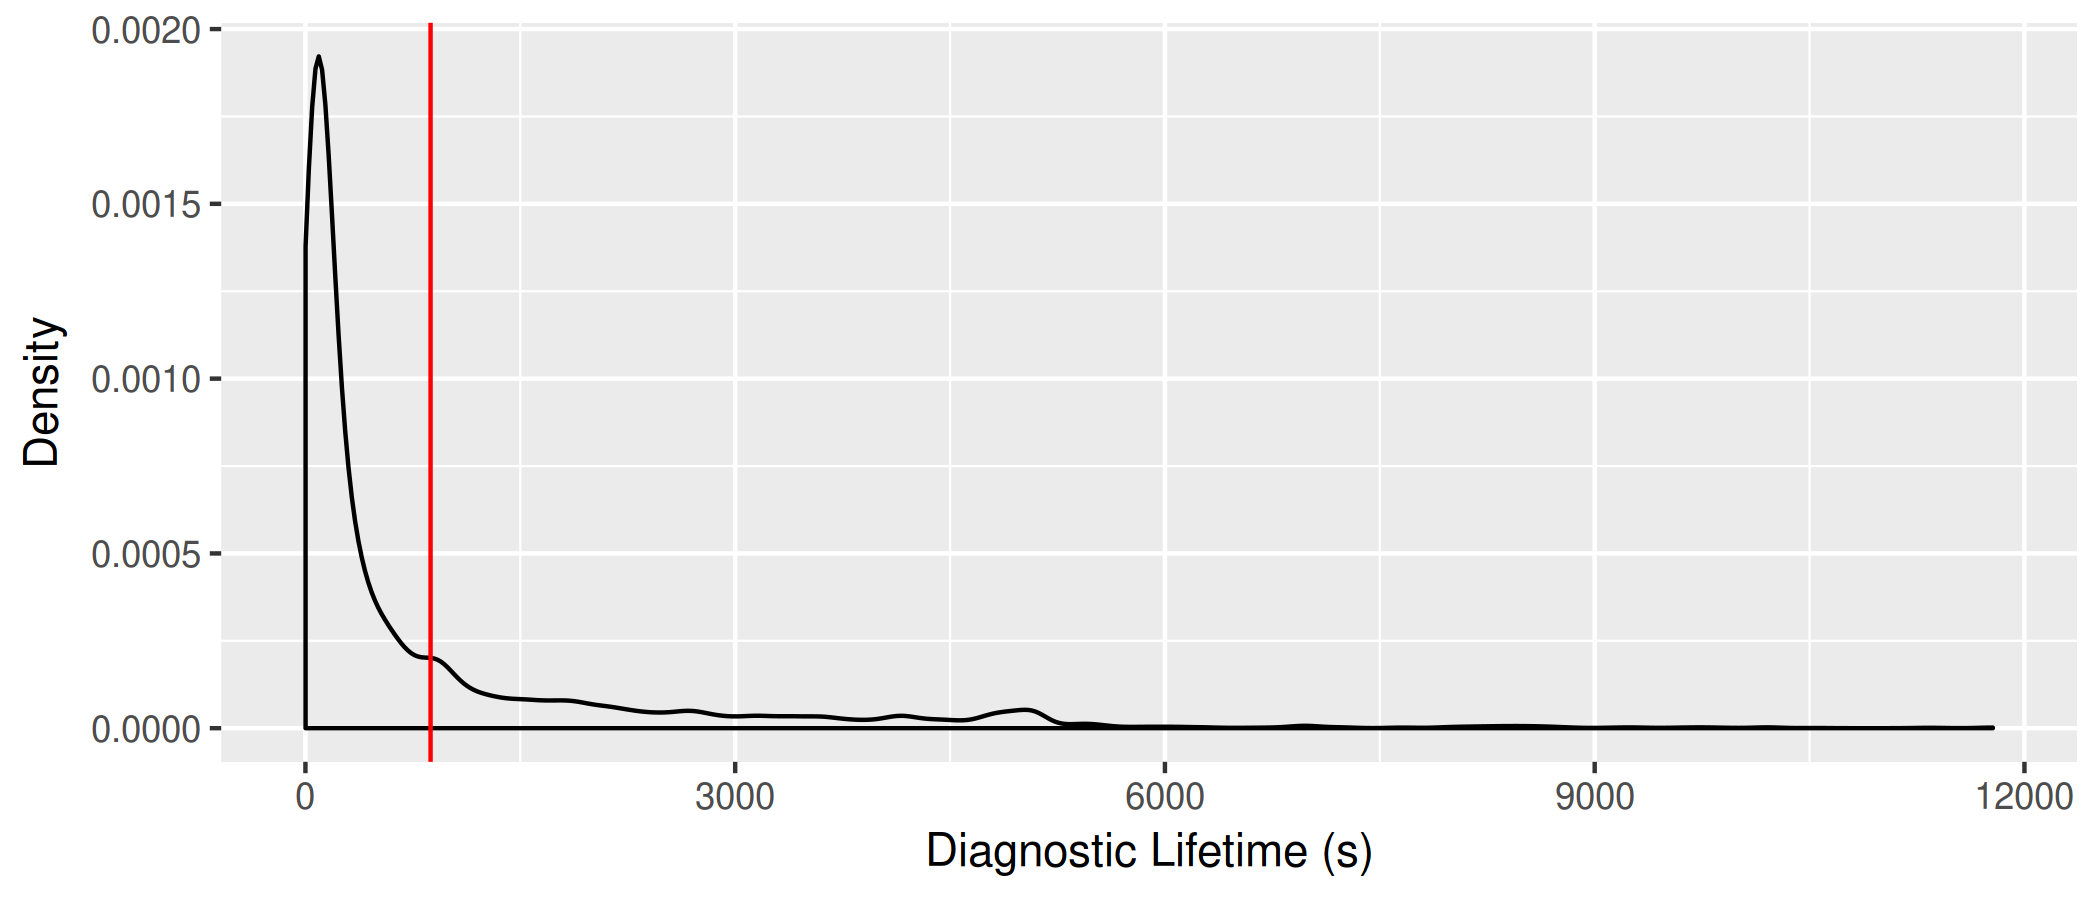
\includegraphics[width=\textwidth]{figures/results/lifetime_density.png}
\caption{Density plot of the diagnostic lifetimes variable.}
\label{fig:avg_lifetime_distribution}
\end{figure}

\begin{figure*}
  \centering
	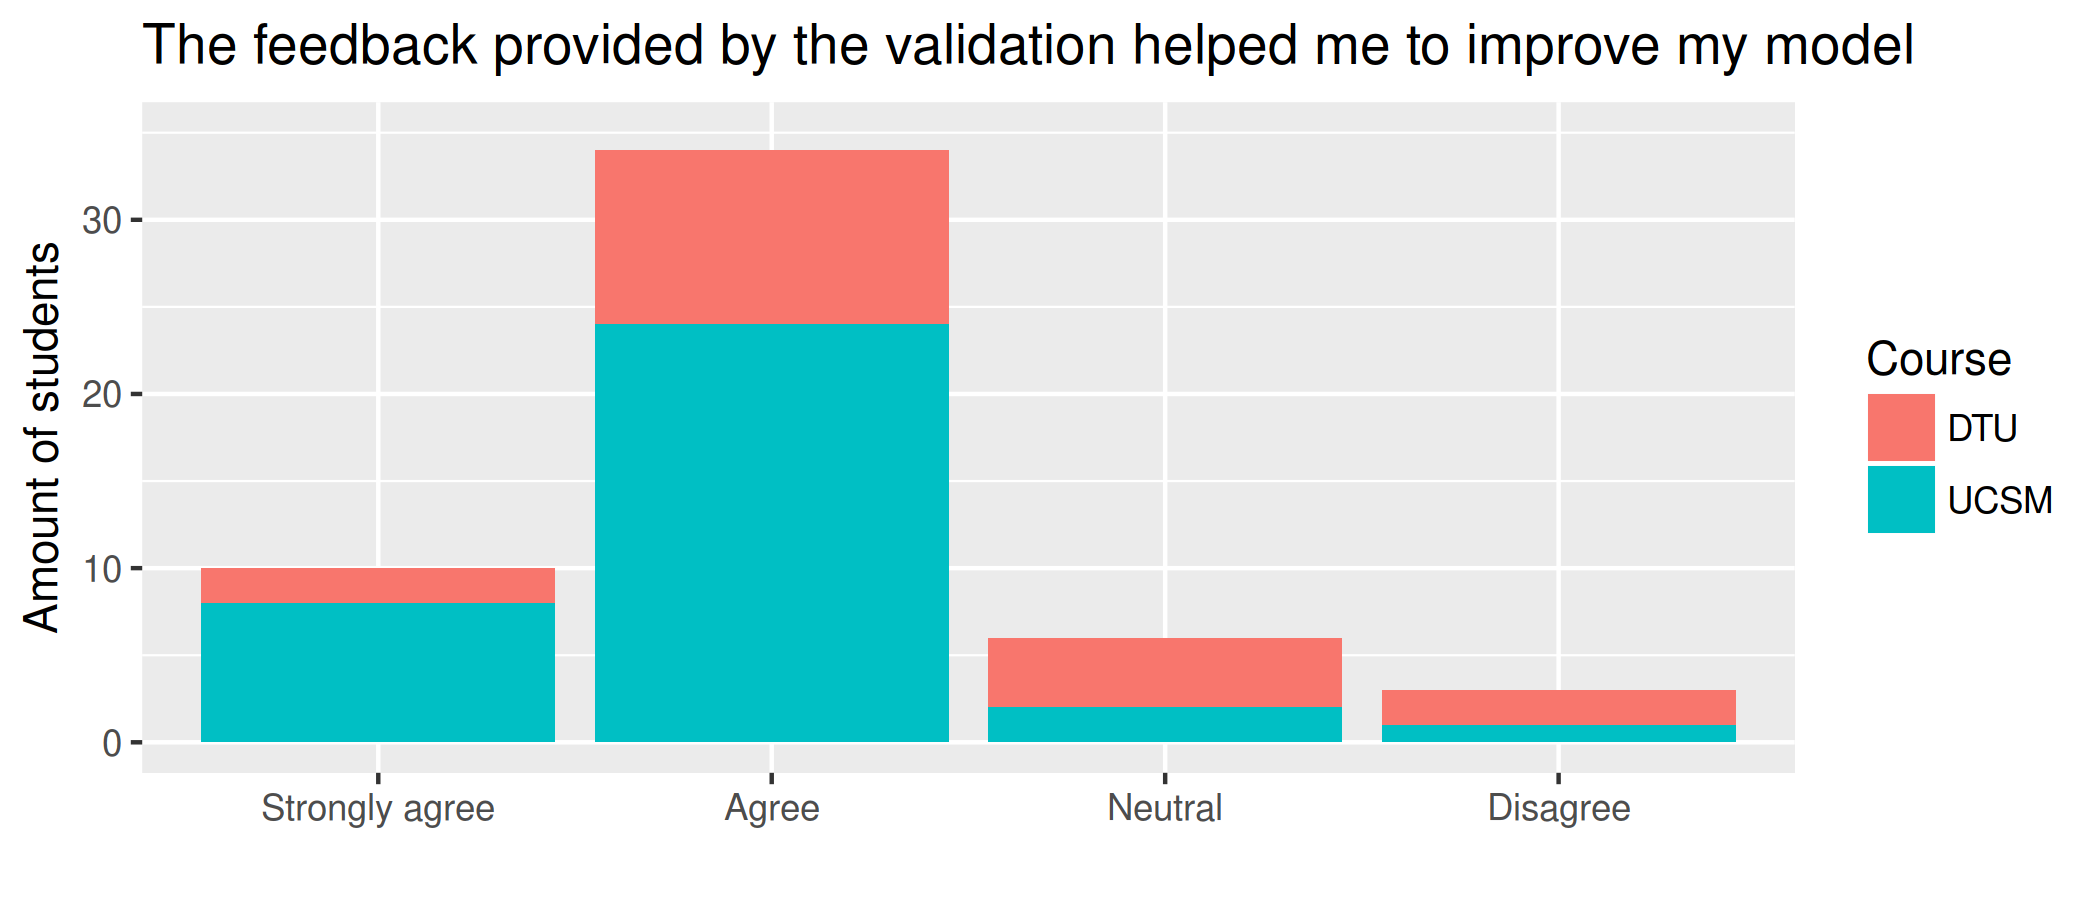
\includegraphics[width=0.9\textwidth]{figures/results/validation_helped_improve}
  \vspace{5pt}
  \newline
  \noindent
	\centering 
	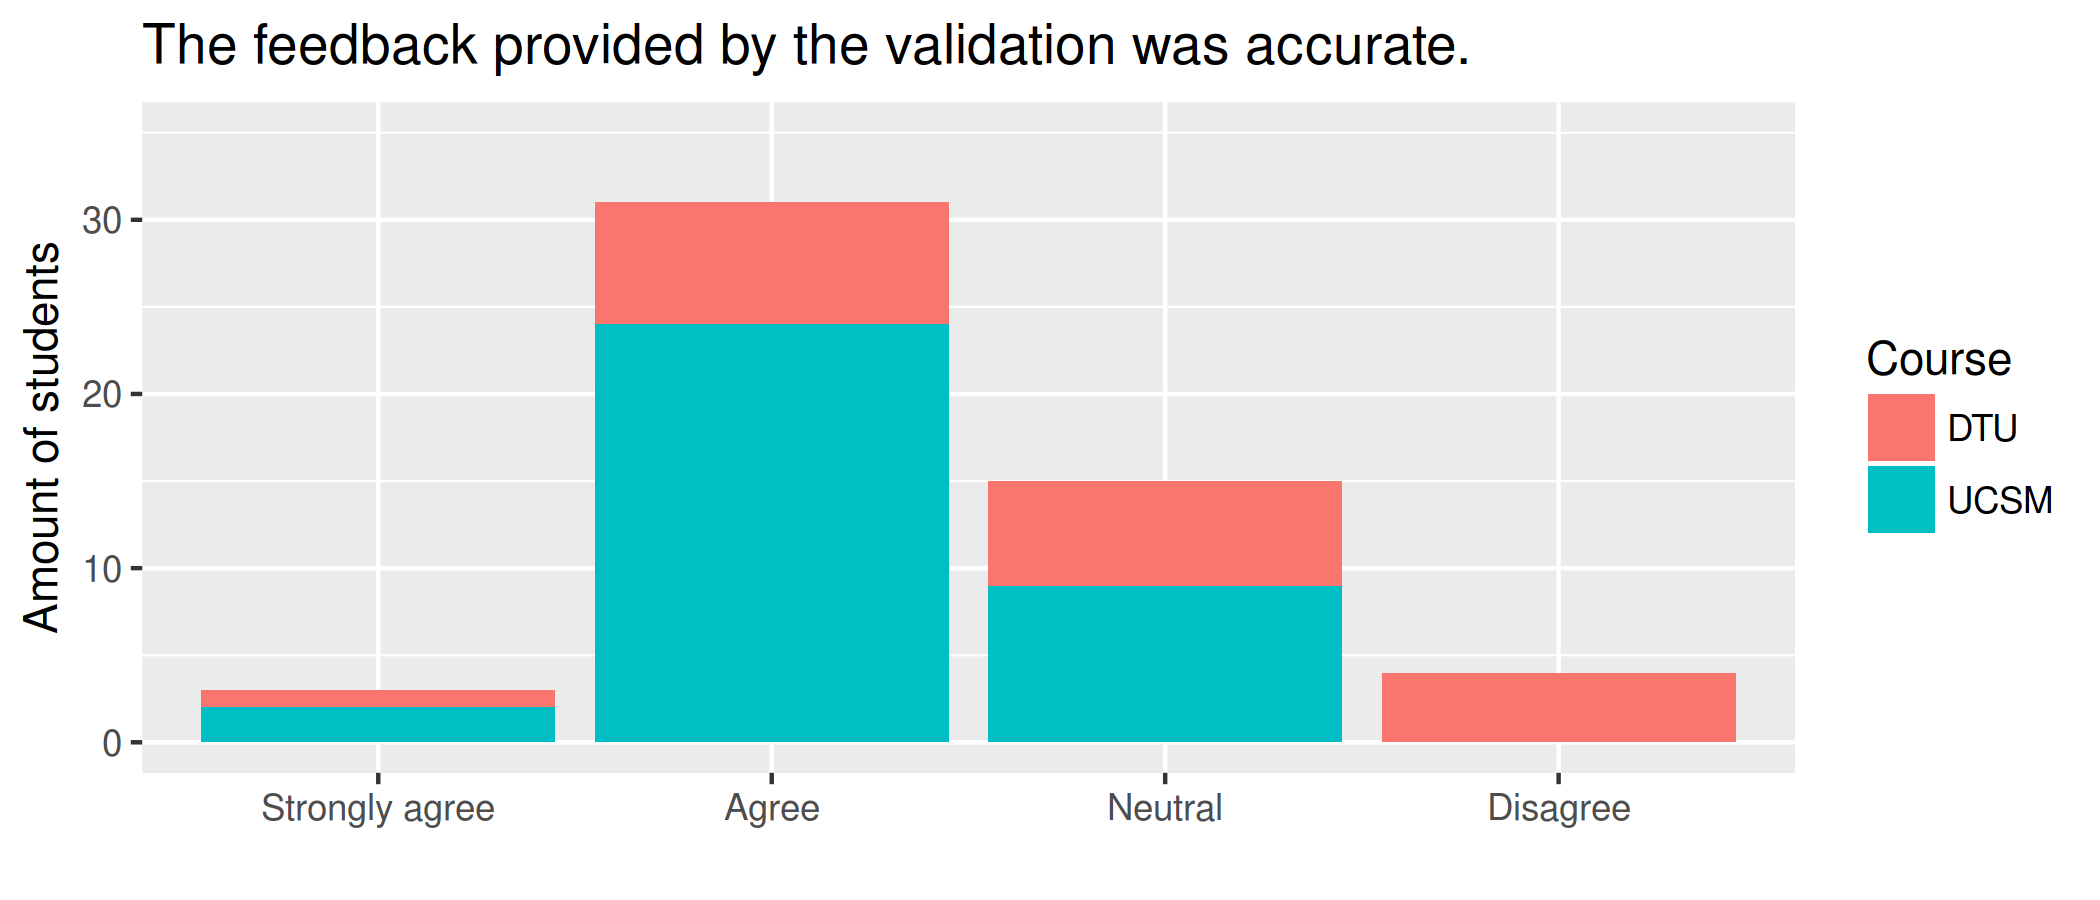
\includegraphics[width=0.9\textwidth]{figures/results/validation_was_accurate}
  \vspace{5pt}
  \newline
  \noindent
	\centering 
	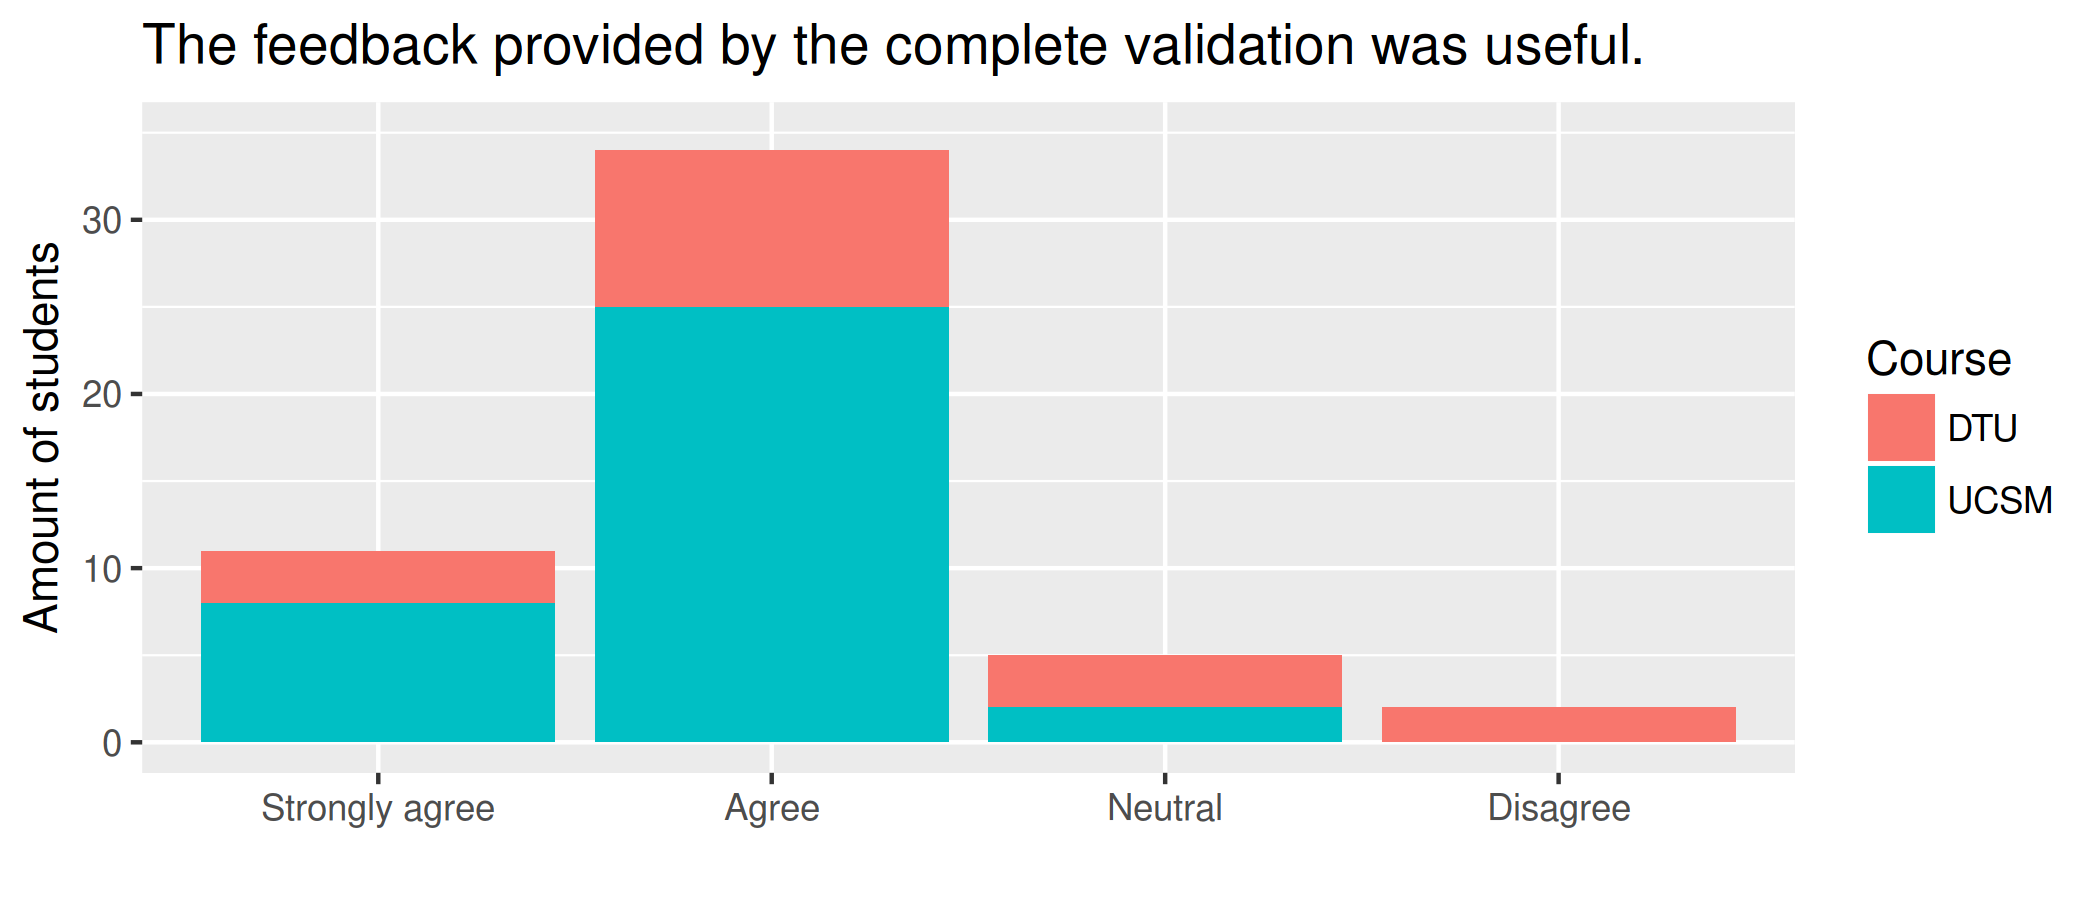
\includegraphics[width=0.9\textwidth]{figures/results/final_was_useful}
  \vspace{5pt}
  \newline
  \noindent
  \centering 
  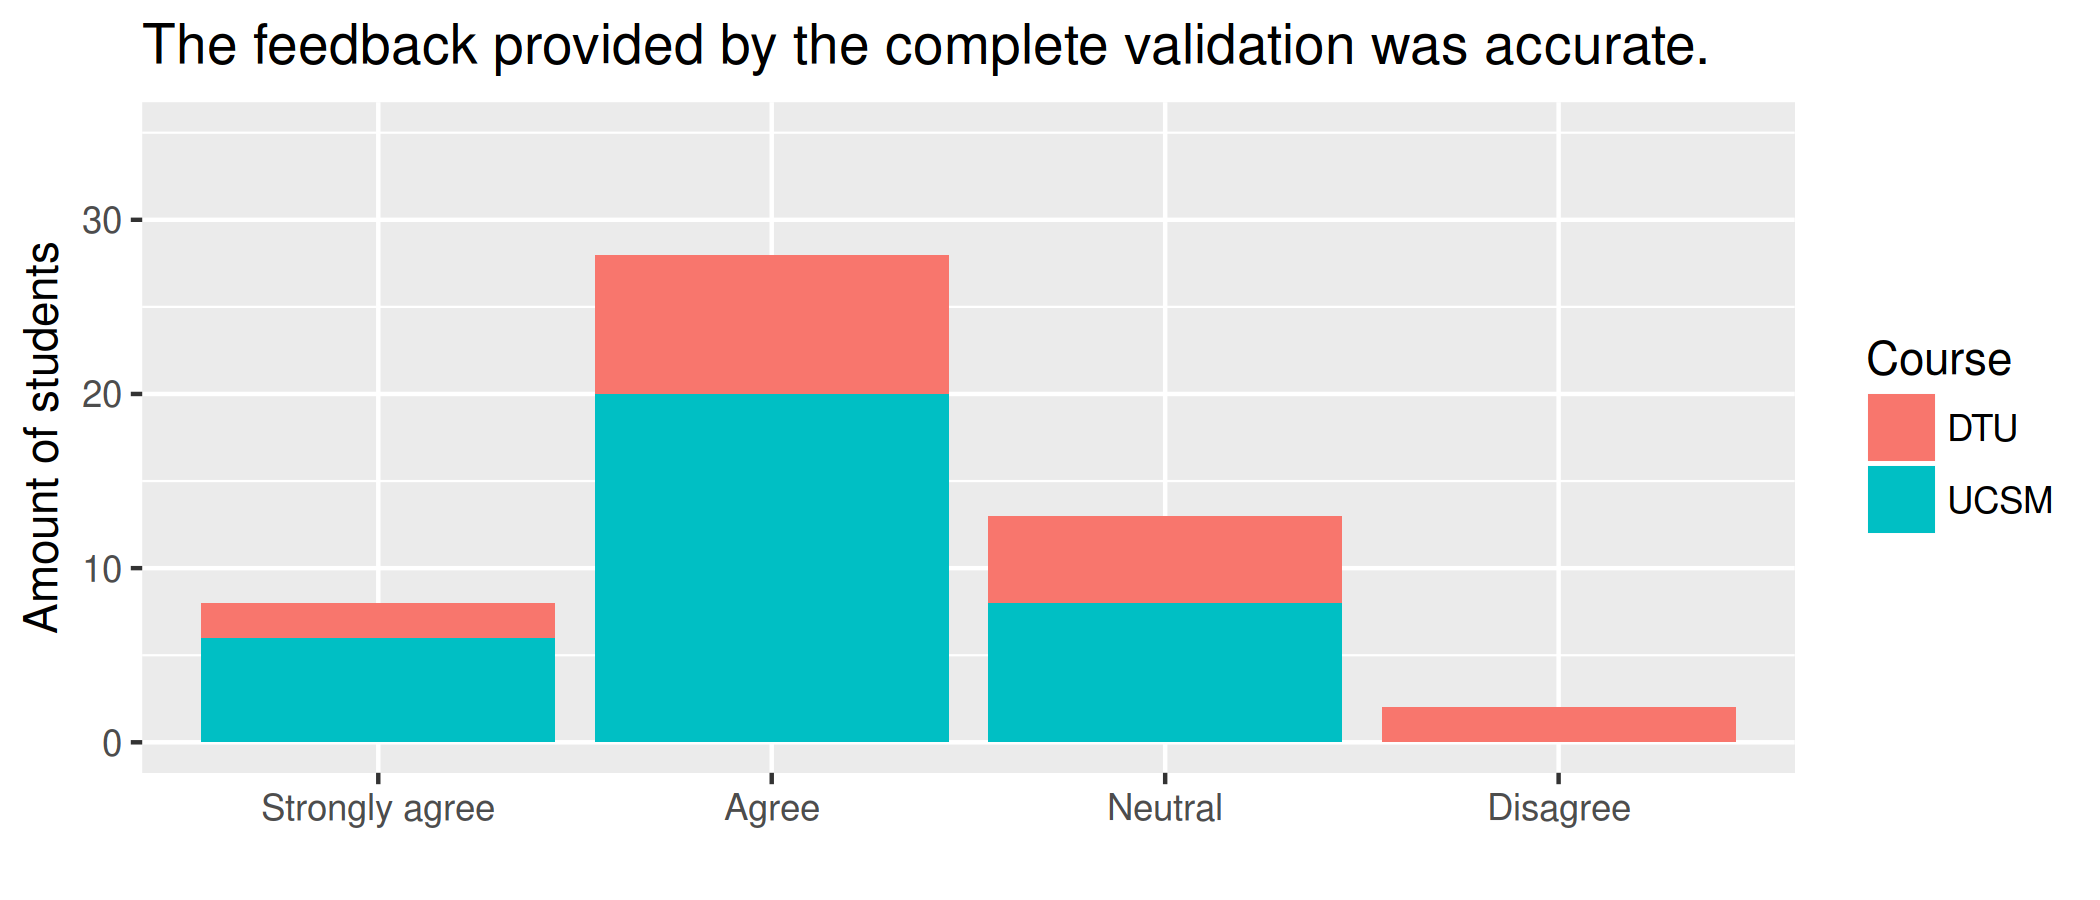
\includegraphics[width=0.9\textwidth]{figures/results/final_was_accurate}
\caption{Results of the student survey for the modeling courses.}
\label{fig:survey-results}
\end{figure*}

\newcommand{\expnumber}[2]{{#1}\mathrm{e}{#2}}

We analyzed how the frequency of different diagnostics varies during the session. Figure~\ref{fig:error_evolution} shows the evolution of the average amount of diagnostics for all students, per diagnostic type. To better observe the relative behaviour of each type regardless of the amount of diagnostics in the category, we plot the values relative to the maximum of each category. We have encountered substantial differences between diagnostic types. 
Missing Activity diagnostics decrease as the session advances, since less activities will be missing as the modeling session progresses.
Unnecessary Activity and Double Action Writing Style increase for the first half of the session, then decrease. This behavior is consistent with the fact that most students do not start using the complete validation feature until the second half of the session. The more detailed feedback of the complete validation then helps them finding the more subtle errors in their process model.


The remaining diagnostic types have an oscillatory behaviour, but still increase for the duration of the session. This can be explained by the fact that, as the model session progresses, there is a greater chance of a student introducing an error leading to one of these diagnostics. However, the drops after 75\% progress could indicate that some students delay the correction of this errors until the end of the modeling session.

%-------------------
\subsubsection{Lifetime of the Diagnostics}
To get a deeper insight into the modeling session data, we computed the lifetime of the diagnostics given to the students. We define the diagnostic lifetime as the elapsed time between the moment a student introduces a mistake in the model, and the moment that mistake is corrected. Note that this metric is independent of the validations made by the student, since diagnostics are computed for all snapshots regardless of the student used the validation function or not.
The average lifetimes follow a long-tailed distribution (Figure~\ref{fig:avg_lifetime_distribution}). That is, in the average case mistakes are quickly corrected by the students. However, for a few cases, it can take a very long time to solve those mistakes. 

%An instructor can use the  information provided in Table~\ref{tab:avg_lifetimes} with several purposes, e.g., to 
%try to improve students understanding of the long-lasting mistakes.

%\todo{[JS: What could we say about the error lifetimes?]}

%\begin{table}
%\begin{tabular}{l|c}
%\hline
%\textbf{Diagnostic} & \textbf{Average Lifetime (s)} \\
%\hline
%Implicit Gateways & 1393 \\
%Gateway Reuse & 418 \\
%Non-Natural Loops & 393 \\
%\hline
%Double Actions Label & 891 \\
%\hline 
%Missing Activity & 2116 \\
%Unnecessary Activity & 367 \\
%\hline
%\textbf{Total} & 873s \\
%\hline
%\end{tabular}
%\caption{Average lifetimes for different error types}
%\label{tab:avg_lifetimes}
%\end{table}







\subsubsection{Relation of Number of Validations and Errors}

Finally, we studied whether there was a correlation between the number of validations performed by the students, and the number of bad diagnostics obtained. To that end, we performed a Pearson's correlation test on the following variables, measured for each modeling session: $V_s =$ ``Number of validations'', $V_c =$ ``Number of \textbf{complete} validations'', $D_{avg} =$ ``Average number of bad diagnostics during the modeling session'', $D_{end} =$ ``Number of bad diagnostics at the end of the exercise''.
\begin{table}
{\scriptsize
\begin{tabular}{l|c c c| c c c }
& \multicolumn{3}{|c|}{\textbf{Correlation Coefficient}} & \multicolumn{3}{|c}{\textbf{Test p-value}} \\
& \textbf{DTU} & \textbf{UCSM} & \textbf{TOTAL} & \textbf{DTU} & \textbf{UCSM} & \textbf{TOTAL} \\
\hline
$V_s$ \textasciitilde $D_{avg}$ & -0.693 & -0.626 & -0.664 & $8.77\times10^{-5}$ & $9.04\times10^{-8}$ & $3.33\times10^{-12}$ \\
$V_s$ \textasciitilde $D_{end}$ & -0.636 & -0.498 & -0.558 & $4.74\times10^{-4}$ & $5.07\times10^{-5}$ & $2.34\times10^{-8}$ \\
$V_c$ \textasciitilde $D_{avg}$ & -0.540 & -0.305 & -0.443 & $4.42\times10^{-3}$ & $1.77\times10^{-2}$ & $ 1.91\times10^{-5}$ \\
$V_c$ \textasciitilde $D_{end}$ & -0.219 & -0.406 & -0.397 & $3.85\times10^{-2}$ & $1.27\times10^{-3}$ & $1.57\times10^-4$ \\
\hline
\end{tabular}}
\caption{Pearson's correlation test results for the relevant pairs of studied variables (shown per course and total).}
\label{tab:correlations}
\end{table}
Besides the obvious correlations $V_c$ \textasciitilde $V_s$ and $D_{avg}$ \textasciitilde $D_{end}$, we also found strong negative correlations between the two pairs of variables, as seen in Table~\ref{tab:correlations}. That is, when the number of validations grows, the number of errors decreases. While all the correlations were statistically significant, we can see how the ones concerning the number of complete validations are weaker than the other two. %This can be explained by the fact that a subgroup of students were told to perform exactly one complete validation. %in one of the exercises. 
This can be explained by the fact that a large group of students did not use the complete validation, or did so only at the end of the session without addressing the feedback, while almost all students used the simple validation.
Additionally, we observed that the correlations found for the individual courses are less strong than considering the 72 students as one group.  

% \todo{[JS: I don't think we should draw very strong conclusions here. The fact that there is a correlation between the number of errors and the number of validations only indicates that the tool \textbf{may} (correlation != causation) help students achieve less errors. However, the statement that our feedback helps the students make better models cannot be drawn from this. The reader has to believe our feedback is accurate and useful (which is, more or less, backed by the surveys) for this correlation to indicate something good. If our feedback were to be counter-productive to model quality, the same correlation would indicate that our tool helps students achieve worse models.]}



\subsection{Student Survey}
\label{sec:questionaires}

In the survey, the students were asked demographical information, native language and line of work, as well as their degree of agreement on some aspects of the application with four questions, aimed at independently evaluating the accuracy and usefulness of the validation and complete validation functionalities. Finally, the students also were asked to write down any complaints and/or improvement suggestions.
% \todo{[JS: I found no interesting correlations with the demographic information so I left it out. Should we include it anyway?]}
Figure~\ref{fig:survey-results} shows the results of the survey: 
%As we can see from the results, 
a majority ($75.4\%$ in average) of students either agreed or strongly agreed in all questions. So we can say that the general perception is that using our framework was beneficial to the students. 
%\todo{[JS: Should we add that the instructors have also found the models to be of better quality with respect to previous years?]}.

When looking separately at the questions regarding \emph{usefulness} versus the ones regarding \emph{accuracy}, we can see a difference, with the students having a stronger level of agreement with the usefulness ($84.0\%$ on average) than accuracy ($67.0\%$ on average). We can thus conclude the student's perception was that the tool was useful, but not as accurate. This can be validated from the student's written suggestions, where in some cases they complained about the tool not understanding their process model labels.

By comparing independently the results of the two modeling courses, we can see the students from DTU were more critical with the tool ($58.3\%$ on average either agreed or strongly agreed) than the ones from UCSM ($83.6\%$ on average). We believe this difference can be partly explained by the presence of some technical issues during the DTU modeling course that were fixed for the UCSM one.


